\chapter{Diseño del proyecto}

En este capítulo se trataran los temas relacionados con la fase de diseño del proyecto, es decir, con el estudio previo que se ha realizado de todos los componentes que se encuentran involucrados en él. En esta agrupación se ve envuelta, por ejemplo, la propia vivienda y su composición estructural, ya que es necesario conocer, entre otros, el espacio físico con que se cuenta para colocar los mecanismos y dispositivos situados en los cuadros eléctricos y domóticos, las dimensiones de las habitaciones para establecer que dispositivos cumplirán correctamente sus funciones o cuales requerirán de una mayor inversión en sus capacidades como pueden ser los sensores de movimiento o los sistemas de aerotermia; e incluso conocer los materiales de paredes y techo para no aportarles una carga superior, tanto de peso como temperatura, humedad o cualquier otra magnitud, a la que podrían aceptar a la hora de instalar y albergar máquinas en su interior sin sufrir ningún tipo de daño.\\\\
Este estudio tomará especial relevancia una vez que el diseño y el desarrollo hayan concluido, y comience la fase de instalación y volcado de las programaciones, donde los elementos deberán ser colocados en sus respectivos puestos y comenzar a funcionar según se les ha indicado. Esto se deba a que en este punto, sin la validación adecuada del diseño previo, podrían presentarse graves problemas que no harían más que encarecer y alargar temporalmente el proyecto, lo que lo alejaría de la meta de que el cliente se encuentre satisfecho con el resultado de la domotización de su vivienda, a la par de resultar económicamente viable para la empresa.


\section{Dimensionamiento del proyecto}

A la hora de diseñar una instalación domótica para una vivienda es importante no pasar por alto una serie de factores restrictivos para que todo el sistema funcione correctamente. Dos de estos parámetros que han de ser tomados en cuenta son el tamaño físico de los módulos y la demanda de potencia que reclaman.\\
 El factor de tamaño viene ligado simplemente a la capacidad de alojar distintos mecanismos que permite el cuadro eléctrico de domótica. En el caso de esta vivienda además, se ha de tener en cuenta la modularidad del sistema, por lo que la opción escogida pasa por duplicar estos armarios, conteniendo cada uno de ellos en su interior los elementos que permitiesen a los subsistemas funcionar de manera independiente en caso de querer dividir la vivienda en dos casas diferentes. El único mecanismo que compartirán ambas viviendas será la fuente de alimentación de 640 mA, por lo que la suma de corriente total no deberá nunca superar este valor. Para realizar este estudio, se han escogido las corrientes máximas que pueden llegar a demandar los mecanismos, en lugar de sus corrientes nominales, cerciorándonos así de que bajo ninguna circunstancia o condición adversa, el sistema quedará sin alimentación por una demanda de intensidad superior a la proporcionada. Para simplificar la visualización de los límites que plantean ambos parámetros, se ha elaborado una lista (tabla \ref{tab:tabla_dimensionamiento}) para facilitar esta tarea:

\begin{flushleft}
\begin{table}[H]
\begin{tabular}{|p{4cm}|c|c|c|c|c|}
\hline 
\rule[0mm]{0mm}{5mm}
\multirow{2}{*}{Descripción}  &  \multirow{2}{*}{Cantidad} & Consumo & Tamaño & Consumo & Tamaño\\
&  &  ud. (mA) &  ud. (DIN) &  Total  (mA) & Total (DIN)\\
\hline
\hline
\rule[0mm]{0mm}{4mm}
Detect. Movimiento &  \multirow{2}{*}{4} &  \multirow{2}{*}{10} &  \multirow{2}{*}{0} &  \multirow{2}{*}{40} &  \multirow{2}{*}{0}\\
Komfort 2,2m KNX& & & & &\\
\hline
\rule[0mm]{0mm}{4mm}
Detect. Presencia  & \multirow{2}{*}{1} & \multirow{2}{*}{10} & \multirow{2}{*}{0} & \multirow{2}{*}{10} & \multirow{2}{*}{0}\\
 KNX Mini Komfort & & & & &\\
\hline
\rule[0mm]{0mm}{4mm}
Detect. Movimiento &  \multirow{2}{*}{1} &  \multirow{2}{*}{10} &  \multirow{2}{*}{0} &  \multirow{2}{*}{10} &  \multirow{2}{*}{0}\\
 KNX Standard 2,2m & & & & &\\
\hline
\rule[0mm]{0mm}{4mm}
\rule[0mm]{0mm}{4mm}
Sensor CO2 +  & \multirow{2}{*}{1} & \multirow{2}{*}{25} & \multirow{2}{*}{0} & \multirow{2}{*}{25} & \multirow{2}{*}{0}\\
Humedad KNX & & & & &\\
\hline
\rule[0mm]{0mm}{4mm}
Pulsador KNX de 2 elem. &  \multirow{2}{*}{37} &  \multirow{2}{*}{5} &  \multirow{2}{*}{0} &  \multirow{2}{*}{185} &  \multirow{2}{*}{0}\\
con mando de 1 punto  & & & & &\\
\hline
\rule[0mm]{0mm}{4mm}
Fuente alimentacion & \multirow{2}{*}{1} & \multirow{2}{*}{-640} & \multirow{2}{*}{4} &  \multirow{2}{*}{(-640*)} & \multirow{2}{*}{4}\\
 640mA KNX  & & & & &\\
\hline
\rule[0mm]{0mm}{4mm}
Actuador de conmutación   &  \multirow{2}{*}{2} &  \multirow{2}{*}{24} &  \multirow{2}{*}{12} &  \multirow{2}{*}{24} &  \multirow{2}{*}{12}\\
24 outs / 12 persianas 16A  & & & & &\\
\hline
\rule[0mm]{0mm}{4mm}
Actuador calefaccion & \multirow{2}{*}{2} & \multirow{2}{*}{12} & \multirow{2}{*}{4} & \multirow{2}{*}{48} & \multirow{2}{*}{8}\\
6 elementos KNX & & & & &\\
\hline
\rule[0mm]{0mm}{4mm}
Entrada binaria KNX de &  \multirow{2}{*}{4} &  \multirow{2}{*}{7,5} &  \multirow{2}{*}{2} &  \multirow{2}{*}{30} &  \multirow{2}{*}{8}\\
 6 elem. 10-230 V CA/CC & & & & &\\
\hline
\rule[0mm]{0mm}{4mm}
 Detector de humos & 4 & 0  & 0 & 0 & 0\\
\hline
\rule[0mm]{0mm}{4mm}
Gira X1 & 1 & 10 & 2 & 10 & 2\\
\hline
\rule[0mm]{0mm}{4mm}
Gira G1 & 1 & 0 & 0 & 0 & 0\\
\hline
\rule[0mm]{0mm}{4mm}
Actuador de regulacion  &  \multirow{2}{*}{4} &  \multirow{2}{*}{15} &  \multirow{2}{*}{4} &  \multirow{2}{*}{60} &  \multirow{2}{*}{16}\\
4 elementos Komfort KNX & & & & &\\
\hline
\rule[0mm]{0mm}{4mm}
Interfaz KNX para &  \multirow{2}{*}{2} &  \multirow{2}{*}{15} &  \multirow{2}{*}{2} & \multirow{2}{*}{30} & \multirow{2}{*}{4}\\
contadores de consumo  & & & & &\\
\hline
\rule[0mm]{0mm}{4mm}
Panel táctil capacitivo con display & 6 & 25 & 0 & 150 & 0\\
\hline
\rule[0mm]{0mm}{4mm}
Actuador de clima con &\multirow{2}{*}{2} & \multirow{2}{*}{10} & \multirow{2}{*}{4,5} & \multirow{2}{*}{20} & \multirow{2}{*}{9}\\
zonificación de 4 zonas   & & & & &\\
\hline
\rule[0mm]{0mm}{4mm}
Medidor de energía  & \multirow{2}{*}{2} & \multirow{2}{*}{17,5} & \multirow{2}{*}{2} & \multirow{2}{*}{35} & \multirow{2}{*}{4} \\
eléctrica KNX KES Plus & & & & &\\
\hline
\hline
\rule[0mm]{0mm}{4mm}
 & & &\textbf{TOTALES}&691 (51*)&75\\
\hline
\end{tabular}
\caption{Dimensionamiento}
\label{tab:tabla_dimensionamiento}
\end{table}
\end{flushleft}

En la tabla anterior (\ref{tab:tabla_dimensionamiento}) aparecen elementos con un tamaño DIN igual a cero, lo que es debido, no a su inexistencia, si no a que son elementos que no se instalarán en el cuadro, sino en otros lugares de la vivienda como en paredes o cajas de aplique, por lo que su tamaño no afectará al dimensionamiento final de los cuadros eléctricos y tendrá una menor repercusión a la hora de su implementación al sistema, ya que cuentan con un tamaño bastante reducido.\\
Otro dato relevante se presenta en el consumo total, donde aparecen dos valores: el de consumo total y entre paréntesis el balance del consumo total, en el que se ha tenido en cuenta la insuflación de intensidad de la fuente, permitiendo así conocer el margen existente en la instalación de cara a la implementación futura de nuevos módulos.

\section{Funcionalidad}

\begin{itemize}
\item \textbf{Iluminación: }en esta sección se agrupan todos los elementos de la vivienda que comparten el mismo desempeño: iluminar, independientemente de si se tratan de luminarias del tipo ON/OFF o del tipo regulable. Cada punto de luz se controlará independiente del resto de puntos, y se podrá hacer desde uno o más de los pulsadores instalados, desde la pantalla del G1 o desde la aplicación del móvil. Se han habilitado mediante programación los llamados servicios centralizados, permitiendo así controlar conjuntos de luminarias como por ejemplo, el centralizado general, que permite apagar todas las luces de la vivienda, permitiendo así al cliente poder salir de la vivienda con la seguridad de no estar malgastando energía, ahorrando de esta manera en su factura eléctrica. \\\\ Para esta sección también se ha hecho uso de los sistemas sensoriales de movimiento, presencia y luminosidad: la luminaria del trastero, las de los pasillos y el hall se encienden de manera automática al detectar movimiento en ellos; en el salón, sin embargo, se ha utilizado un detector de presencia al no tratarse de una zona de paso, que en combinación con la cuantificación de luminosidad en la estancia, enciende de manera automática la lámpara si detecta a alguna persona y la regula en función del valor de luminosidad sensado.\\
\item \textbf{Recuperador de CO\textsubscript{2}: }esta sección contará con un detector de partículas de CO\textsubscript{2}, que activará la señal para dar la orden a un sistema de extracción y renovación de aire mediante un sistema de ventiladores. De manera habitual, el sistema de recuperación debe permanecer en funcionamiento con el menor nivel de ventilación activado, y deberá ser apagado y reactivado por el cliente de manera manual mediante un switch habilitado tanto en la G1 como en la aplicación del móvil. \\ 
Si el sistema se encuentra operativo, el sensor lanzará señales de activación de los diferentes niveles de velocidad de los ventiladores en función de la cantidad de partículas detectadas. Concretamente, se han programado tres límites: el primero de ellos, cuando se detectan entre 500 y 1000 partículas de CO\textsubscript{2} por millón analizadas, un segundo limite que activa el siguiente nivel de velocidad de los ventiladores cuando detecta entre 1000 y 1500 partículas por millón, y finalmente el tercer limite, que activa la máxima velocidad al detectar una cantidad superior a las 1500 partículas por millón. Por añadidura, al activar cualquier luz de alguno de los baños, el ventilador entrará en velocidad máxima durante 10 minutos, independientemente de los valores sensados, al igual que al accionar una de las teclas de los pulsadores, que ha sido programada para lanzar esta función de recuperación.\\
\item \textbf{Seguridad ante incendios: }esta sección contará con detectores de humo instalados en diferentes habitaciones de la vivienda, que una vez activados, enviarán una señal de activación a la sirena de alarma y cortarán el suministro de gas mediante el cierre de la electroválvula. Esta alarma enviará una notificación tipo Push a los dispositivos móviles conectados con la instalación, permitiendo la desactivación de la señal acústica, manteniendo el cierre de la electroválvula.\\
\item \textbf{Seguridad ante intrusiones: }para evitar en la medida de lo posible la irrupción de personas no deseadas en la vivienda, esta sección hace uso de los sensores de movimiento y presencia utilizados en la sección de iluminación, para lanzar la señal de alarma que activa la sirena y envía un mensaje Push a los dispositivos móviles conectados con la aplicación.\\
\item \textbf{Seguridad ante inundaciones: }esta sección tendrá un funcionamiento similar a la referida a seguridad frente incendios, únicamente cambiarán los sensores de humo por otros de inundación, que estarán ubicados en las zonas húmedas de la casa, como son los baños y la cocina.\\
\item \textbf{Clima:} esta sección será la encargada de controlar la temperatura de la vivienda haciendo uso de diversos elementos. Entre ellos encontramos los termostatos, que harán las veces de interfaz con el usuario en cada habitación gracias a sus pulsadores y displays, permitiendo controlar la velocidad de los ventiladores en caso de que se encuentren en funcionamiento, controlar si se desea o no aclimatar esa estancia y que temperatura es la requerida por el cliente. Internamente, también se encargará de gestionar al resto de equipos, indicando cuando y como deben encenderse y actuar en función de la temperatura sensada y la temperatura de consigna deseada. \\
Durante el verano, el equipo de refrigeración se basará únicamente en el uso del equipo de fancoil, evitando así la aparición de hongos y humedades producidos por la condensación proveniente del uso del suelo radiante. El usuario podrá elegir entre dos modalidades de actuación: la manual, en la que podrá seleccionar entre tres niveles la velocidad a la que desea que se expulse el aire refrigerado en el equipo fancoil, o bien el modo automático, en el que el módulo de actuación de las rejillas seleccionará de entre las tres velocidades mencionadas anteriormente una de ellas en función de un factor de ponderación. Este factor, limitado a un máximo de 100 puntos, será implementado durante su programación, dotando de un valor numérico a cada habitación en función de diversos parámetros como pudiera ser su tamaño o el nivel de confort que requiera. Un ejemplo claro de esto pudiera ser la actuación de uno de los equipos instalados que se encargaría de controlar la temperatura de la cocina, el salón y una de las habitaciones, a los que se les ha otorgado una ponderación de 15 puntos, 55 puntos y 30 puntos respectivamente. Si en una primera situación, hubiese demanda de la cocina y la habitación, al sumar 45 puntos no llegarían al requerimiento del segundo nivel de velocidad, activando así el primer nivel; mientras que si se activasen cocina y salón simultáneamente, al superar el baremo, sí que entraría en funcionamiento la segunda velocidad del equipo.
\bigskip
\begin{table}[H]
\begin{center}
\begin{tabular}{| c | c |} \hline
\rule[0mm]{0mm}{6mm}
\textbf{Valor ponderado de demanda} & \textbf{Nivel activo} \\ \hline
\rule[0mm]{0mm}{3mm}
0 & OFF \\ \hline
\rule[0mm]{0mm}{3mm}
1-33 & Velocidad 1 \\ \hline
\rule[0mm]{0mm}{3mm}
34-66 & Velocidad 2 \\ \hline
\rule[0mm]{0mm}{3mm}
67-100 & Velocidad 3 \\ \hline
\end{tabular}
\caption{Ponderación velocidad fancoils}
\label{tab:vel_fancoils}
\end{center}
\end{table}
En cambio, durante el modo invierno el equipo principal que actuará será el de suelo radiante. En este caso el termostato se encargará de enviar una orden de apertura a las válvulas de las habitaciones en las que la temperatura se encuentra por debajo de la demanda, y una señal de arranque a la caldera en cuanto que una de estas válvulas es abierta, haciendo circular el agua caliente a través del entramado de tuberías instaladas en el suelo. En el momento que la temperatura de la habitación y la de consigna tienen una diferencia mayor de 3ºC, se ha programado el comienzo de actuación del sistema secundario: el sistema de fancoil. El sistema de aerotermia tendrá exactamente el mismo modo de funcionamiento que en el modo verano, activando sus velocidades en función de la ponderación de las habitaciones que se encuentren en demanda al encontrarse funcionando en modo automático, o pudiendo ser elegida por el usuario en el modo manual. \\\\
Para evitar el uso prolongado e indebido de los equipos que componen el sistema, se han programado un control del tipo proporcional integral (PI), debido a que se ajusta mejor al comportamiento que este ofrece frente a la alternativa del control de dos puntos con histéresis. Se trata de un método de control regido por un algoritmo de control lineal basado tanto en la diferencia entre las temperaturas de consigna y de referencia como en los datos del histórico del sistema, reduciendo así las franjas de oscilación de la temperatura del habitáculo, estabilizando paulatinamente su valor en el entorno de la temperatura de consigna establecida por el usuario. \\\\
Como se puede apreciar en la Imagen \ref{fig:metodos_control}, se ofrece una comparativa entre los dos métodos de control para que el sistema proporciona a la estancia una temperatura de 25ºC. Por el método, descartado, de control mediante dos puntos se establecen los límites inferior y superior de temperatura en los que el sistema debe encenderse y apagarse, respectivamente. Con este método más sencillo de programar, el sistema no se encuentra funcionando constantemente, pero sufre picos de alto consumo energético para alcanzar el límite superior desde una temperatura ligeramente menor al límite inferior, con el añadido de que la estancia se encuentra, casi en la totalidad del tiempo, lejos de la temperatura de consigna. En cambio, el método de control proporcional integral, se encuentra constantemente en funcionamiento y trabaja regulando la temperatura de exhalación del aire para mantener la temperatura en un valor más ajustado al de consigna de manera constante, sin provocar tiempos de funcionamiento a marchas forzadas de la máquina de aerotermia o de la caldera, evitando así los picos de alta demanda energética por parte del sistema. 
\bigskip
\begin{figure}[H]
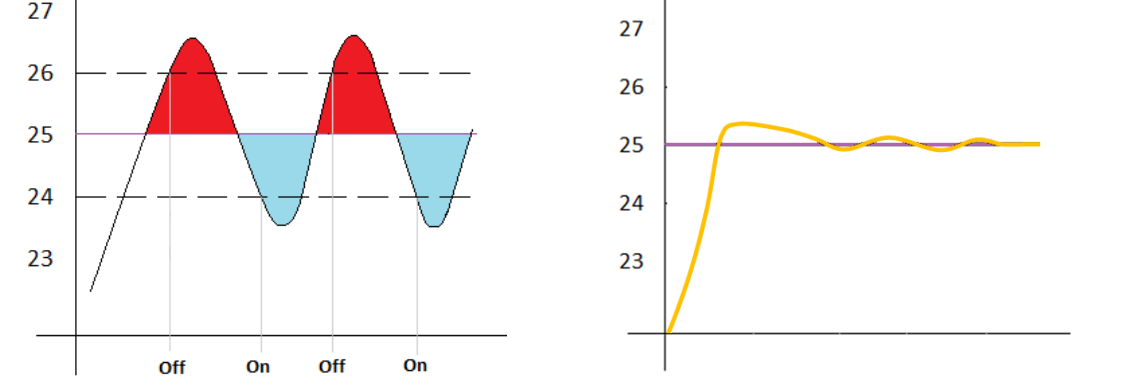
\includegraphics[width=1.15\textwidth]{figures/metodos_control.png}   
\caption{Comparación entre control de dos puntos con histeresis [izq] y control PI [dcha]}
\label{fig:metodos_control}
\end{figure}
\bigskip
La programación de este algoritmo requerirá de la configuración de tres parámetros esencialmente:
	
	\begin{itemize} 
	\item La constante de proporcionalidad (K) expresada en grados centígrados, encargada de que el error estacionario se 	reduzca a cero produciendo el menor valor posible de sobreoscilación de la señal. 
	\item El tiempo integral (T) expresado en minutos, será un valor asociado a la inercia térmica del sistema de aerotermia que 				permite ajustar el error de aproximación en función del tiempo transcurrido, es decir, la velocidad de impacto que tiene el 	sistema para variar la temperatura.
	\item El tiempo de ciclo, también expresado en minutos, que condicionará la frecuencia de muestro y actualización de la señal de 			control enviada tanto a la caldera como a las máquinas de aerotermia.
	\end{itemize} 
Se ha establecido un valor de K=4 y T=90min. tanto para el modo enfriar como calentar de la máquina de aerotermia, mientras que para el suelo radiante, los valores escogidos han sido K=5 y T=240min. El tiempo de ciclo que se ha encontrado más optimizado respecto a las condiciones de ahorro energético y confort térmico ha sido de 15min. \\
El control de los sistemas de fancoil normalmente se ejecuta a través de comunicaciones vía infrarrojos, protocolo que no entra dentro del alcance de la tecnología KNX, por lo que ha sido necesaria la implementación de un sistema de pasarelas para poder establecer el nexo de comunicación entre el equipo y el bus KNX de manera remota, sin uso de señales infrarrojas. Esta pasarela será conectada al mando de control original de la máquina de aerotermia, que no será removido de la instalación debido a su alta fiabilidad a la hora de identificar los posibles errores o fallos que sufra el equipo. Adicionalmente, el cliente tendrá la opción de cambiar entre modo invierno/verano desde la pantalla del G1 o desde la aplicación del móvil, en función de si desea que el sistema proporcione calor o frio, respectivamente.\\

\item \textbf{Consumos:} por petición del cliente, se debe hacer un seguimiento de los consumos tanto de luz, como de agua y gas que se dan en la vivienda, por lo que se han habilitado lectores adicionales a los respectivos instalados por las compañías de suministro, permitiendo visualizar en la pantalla del G1 o en la aplicación del móvil el consumo instantáneo de tensión, corriente, potencia, agua o gas; el consumo total de energía, de agua y gas durante diversos periodos, como por ejemplo el consumo del mes anterior, el consumo desde el día 1 del mes en el que se encuentren o incluso en un periodo definido por el propio usuario.
\end{itemize} 

\section{Ubicación}

Otro factor (esta en el word)...\\\\\\
La ubicación respecto del resto de elementos de la vivienda también es un factor a tener presente a la hora de realizar el diseño previo de la instalación, ya que de no tenerse en cuenta podría dar lugar a funcionamientos inesperados, la inhabilitación del mecanismo o llegar incluso a provocar situaciones de peligro para el usuario. El caso del detector de humos es uno de ellos, y es que una colocación incorrecta podría dar lugar a que el sensor no detectarse los cambios en la temperatura de la habitación o que al contar esta con grandes dimensiones, no fuese capaz de detectar la presencia de humos nocivos para la salud adecuadamente. Es por ello que, y siguiendo las recomendaciones del fabricante, estos sensores deberán colocarse en el centro de una habitación no más grande de 60 m\textsuperscript{2} y a una distancia mínima de 50 centímetros  otros elementos como lámparas o paredes, sin superar los 6 metros de altura. \\\\
Los detectores de inundación también deberán ser instalados siguiendo una serie de pautas para asegurar su correcto funcionamiento. Entre otras normas, se puede destacar que debe colocarse de manera sobre una superficie que no tenga una inclinación demasiado pronunciada, siendo óptimo que esta sea totalmente horizontal y al nivel más bajo posible de altura tal y como se muestra en la imagen \ref{fig:local_inundacion}, debido a que será necesario el contacto físico entre el sensor y el elemento líquido para hacer saltar la alarma. Es importante también una situación de cercanía con las fuentes de caudal y los electrodomésticos o elementos sobre los que se desea hacer el control, ya que la detección de la fuga será más temprana. Pese a su reducido tamaño, se deberá contar con el espacio que ocuparán estos sensores a la hora de la planificación.\\\\
\begin{figure}[H]
\begin{center}
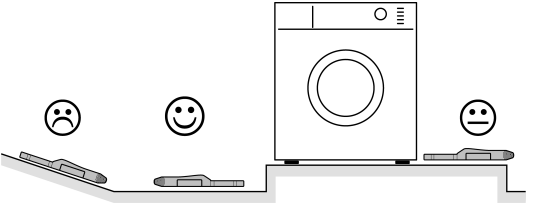
\includegraphics[width=0.85\textwidth]{figures/local_inundacion.png}   
\caption{Ejemplos de posicionamiento de los sensores de inundación}
\label{fig:local_inundacion}
\end{center}
\end{figure}
Otro ejemplo de la importancia de la ubicación de los elementos la encontramos en los sensores de movimiento de tipo PIR: la geometría de la lente que lo recubre le permite detectar la radiación térmica con un amplio margen de amplitud, unos 180º aproximadamente. Esta capacidad será aprovechada al máximo siguiendo una serie de criterios como, por ejemplo, la altura a la que se encuentre y la posición en la habitación respecto de otros enseres que en ella se encuentren. Según las indicaciones del fabricante, el sensor debe ser colocado a una altura de 2,20 m con una leve inclinación hacia el suelo, permitiendo así una mayor dispersión de los haces detectores por la sala. También es necesario tener en consideración el tipo de movimiento que se va a realizar en las salas donde van a ser instalados, ya que el alcance de estos sensores varía en función de si se trata de un movimiento de tipo radial o tangencial.
\begin{figure}[H]
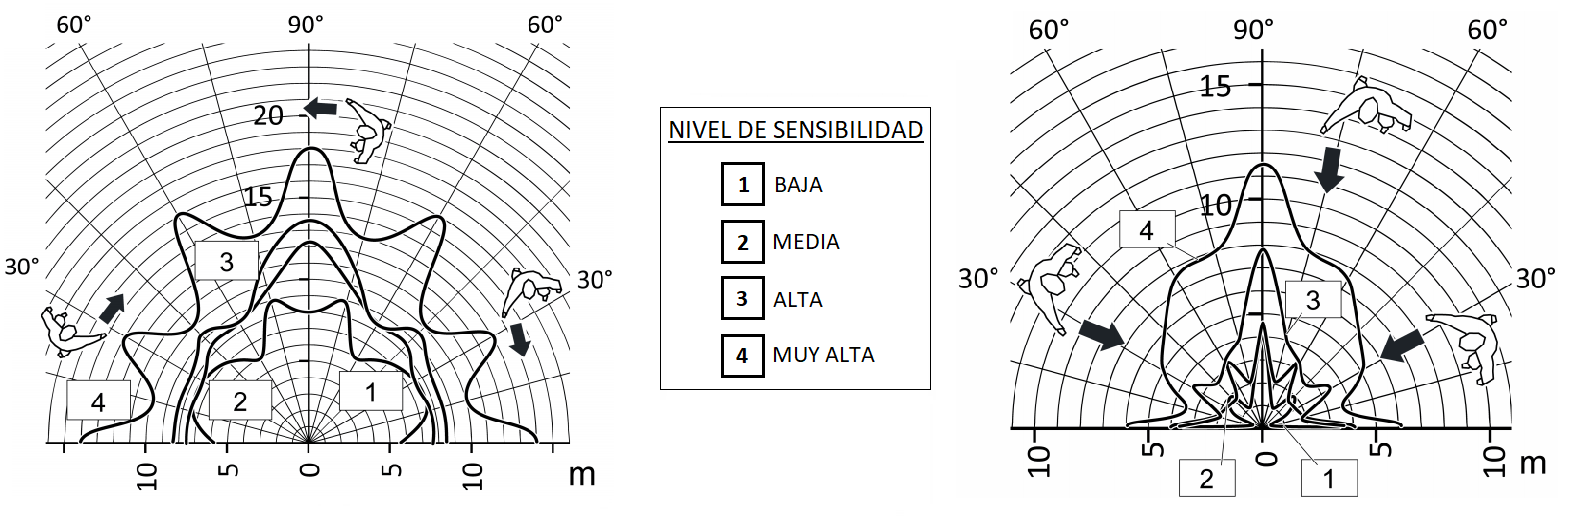
\includegraphics[width=1.15\textwidth]{figures/alcance_PIR.png}   
\caption{Alcances del sensor PIR para movimiento tangencial [izq] y radial [dcha]}
\label{fig:alcance_PIR}
\end{figure}

Como la función que tienen asignada estos sensores es la de detectar el movimiento en los pasillos y el hall de la vivienda para activar la orden de encendido de las luces, se han colocado estratégicamente en los extremos de los pasillos, aprovechando su alta sensibilidad ante el movimiento tangencial, que es el más usual en este tipo de espacios. En cuanto a los sensores que se encuentran en el hall y el trastero, se han situado en lo alto de las paredes situadas enfrente de las puertas de acceso, para encender las luminarias en el momento que estas son abiertas.\\
En el caso de detector de presencia instalado en el salón se cuenta con un radio de detección de 360º, por lo que será instalado en el centro del techo de la sala. Al tratarse de una vivienda antigua, el techo se cuenta con una altura considerable (~3,50m), lo que supondrá una ventaja, ya que de igual manera que los sensores de movimiento, al colocarse en una posición más elevada, se obtiene una mayor distancia de detección, siempre teniendo en cuenta el tipo de movimiento que se desee detectar:
\begin{figure}[H]
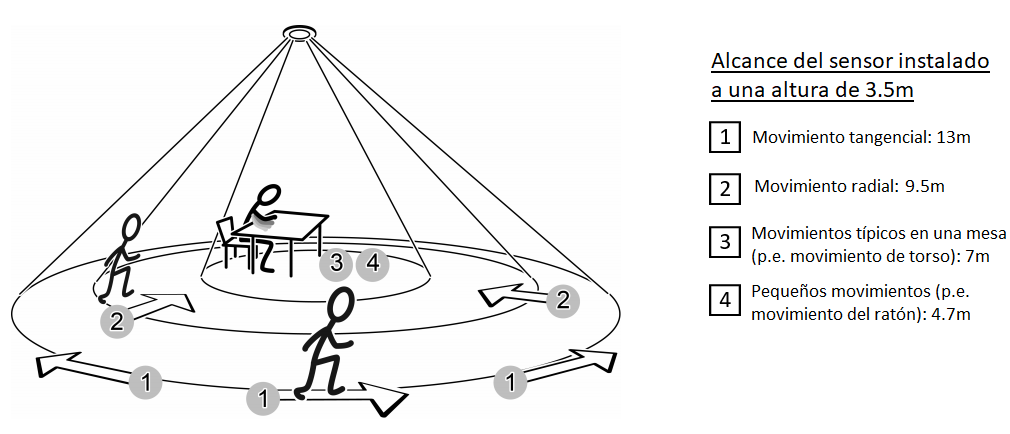
\includegraphics[width=1.15\textwidth]{figures/alcance_presencia.png}   
\caption{Alcances del sensor de presencia}
\label{fig:alcance_presencia}
\end{figure}

\section{Conexionado}
En esta sección...\\\\\\\\
\begin{itemize}
\item \textbf{Cuadro eléctrico de domótica } \\ \\
Siguiendo las normas de seguridad recogidas en la normativa \cite{Reglamento:2021}, una de las líneas del sistema trifásico y el neutro de la instalación eléctrica del edificio se hacen pasar en primera instancia por un Interruptor General Automático (IGA), ya que el Interruptor de Control de Potencia (ICP), encargado de cortar el suministro en situaciones de sobrecarga, cortocircuito y en los que la demanda de potencia supera a la potencia contratada, se encuentra integrada en el contador instalado en la vivienda por la compañía de suministro eléctrico. El IGA tendrá como misión principal proteger el resto del circuito en el caso de que se produzca un cortocircuito o se supere la potencia máxima que es capaz de soportar la instalación, como por ejemplo, cuando son conectados demasiados electrodomésticos a la vez. Esta interrupción de la corriente nada tendrá que ver con cuestiones económicas o limitantes en función de lo que se tenga contratado y se pague a la compañía de suministro eléctrico, si no que será limitante en cuanto a las características físicas de la propia instalación, no pudiendo ser mejorada si no son sustituyendo y mejorado alguno de los elementos que la componen. A continuación, se ha instalado un Protector Contra Sobretensiones (PCS), que tal y como indica su nombre será el encargado de proteger el resto de circuitos en las ocasiones en las que se produzcan picos elevados de tensión no controlados, como puede ser el caso del impacto de un rayo, desviando la corriente hacia la toma de tierra, evitando daños en los equipos conectados, en la propia instalación o incluso sobre los usuarios que se encuentran en el interior de la vivienda.\\\\
Siguiendo el cableado, el siguiente elemento que nos encontramos es el Interruptor Diferencial (ID). Este elemento desarrollará la función de proteger a los usuarios de las fugas de corrientes a tierra que pudiesen producirse por daños o malas conexiones de los electrodomésticos con la instalación eléctrica. En cada vivienda es usual instalar entre dos y tres ID que agrupen varios sistemas con diferentes funcionalidades, facilitando así localizar que la fuga de corriente se está produciendo en alguno de los elementos que a ella se encuentra conectado, pero debido a demanda del cliente, se ha seguido el modelo habitual de instalación aplicado en los cuadros de las viviendas de Alemania, en el que existe un ID por cada una de las funcionalidades que se desarrollan en la instalación, teniendo el sistema de iluminación su propio ID, por ejemplo. \\\\
En último lugar, y antes de comenzar conectar los elementos, se colocan los últimos elementos de protección del sistema: los Pequeños Interruptores de Potencia (PIA), o como son conocidos comúnmente, Interruptores Automáticos. Estos interruptores sí que es habitual encontrarse uno por cada grupo de elementos con la misma funcionalidad, y tendrán como misión detectar el exceso de consumo en estos grupos, desconectándose de manera automática en tal caso. También son muy útiles en el caso de querer realizar alguna modificación en un sistema concreto, ya que si es preciso desconectarlo, no afectará al resto, que podrán seguir operando de manera normal.
\end{itemize} 
Una vez explicado el conexionado hasta el cuadro de domótica, se entrara en detalle el cableado de este hasta los módulos y mecanismos que componen la instalación domótica que controla la vivienda. Entre ambas partes, se han utilizado dos tipos distintos de bornas para facilitar el peinado de los cables, su distribución y organización a lo largo de los tubos y debido a que la ley vigente dictamina que no es legal ni seguro la conexión directa de cables, teniendo que realizarse está a través de algún elemento de paso y sujeción: las bornas de paso y las de distribución. Para una mayor claridad, las bornas de distribución vendrán representadas en los esquemas con un color verde, y serán utilizadas, tal y como su nombre indica, para distribuir las tensiones que llegan a los PIAs. Estas bornas cuentan con cuatro puertos interconectados entre ellos, ofreciendo así el mismo valor de tensión en cada una de sus salidas y son independientes unas bornas a otras, a menos que se haga una conexión directa entre alguno de sus puertos. \\
Por otro lado, las bornas de paso, representadas en color amarillo, también cuentan con cuatro puertos, pero en esta ocasión no se encuentran conectados entre ellos, si no que tienen una distribución distinta, tal y como se muestra en la imagen. En estas bornas, el segundo y cuarto puerto si cuentan con una conexión interna para así ofrecer la misma caída de tensión en ambos puntos, mientras que el primero y el tercero serán independientes. Estas salidas cuentan con conexiones laterales que les permiten conectarse a la borna contigua al encontrarse enganchadas físicamente unas a otras, sin necesidad de realizar esta conexión mediante cables. Por lo tanto, una fila de bornas de paso compartirá la misma tensión con el resto en su primer y tercer puerto, que serán los asignados a la toma de tierra y al neutro común, respectivamente. Los otros dos puertos, serán independientes del resto de bornas e irán conectadas a la fase, uno de ellos a la entrada desde el actuador y el otro al elemento que se desea controlar.

\begin{itemize}
\item \textbf{Actuadores reguladores y binarios y de persianas} \\ \\
Una vez explicado el conexionado hasta el módulo, se pasa a detallar el cableado desde este hasta el elemento a controlar. Para esta sección, se ha dividido los elementos en tres bloques en función de su conexión: en el primer bloque se encuentran todos los elementos de tipo On/Off conectados al actuador de 24 salidas, al que llegará la fase a una de sus salidas desde la borna de distribución, saliendo por el otro terminal de esa misma salida hacia la borna de paso. La conexión de estos elementos será muy simple: de la borna de paso alimentada con fase saldrá uno de los cables que irán al elemento en cuestión, volviendo desde el otro terminal al puerto del neutro de la borna. Para el segundo tipo de elementos el conexionado será idéntico a los del primer tipo, pero en esta ocasión el actuador no solo permitirá abrir o cerrar el circuito, si no que permitirá regular la corriente de salida, realizando así la función de dimmer. Por ultimo tenemos los elementos tipo ventana, que necesitaran de dos de las salidas del actuador de 24 salidas, que vendrán alimentadas desde la borna de distribución, y saldrán hacia la borna de paso. En esta ocasión, de la borna de paso será necesario sacar tres cables hacia el elemento: uno de ellos llevara el neutro, mientras que los otros dos irán conectados a los terminales que determinan si el motor de la persiana o ventana debe actuar en una dirección o su contraria. Todas estas órdenes serán transmitidas a través del cable de bus KNX al actuar sobre los pulsadores, la pantalla o la aplicación móvil.
\end{itemize}

\begin{flushleft}
\begin{figure}[H]
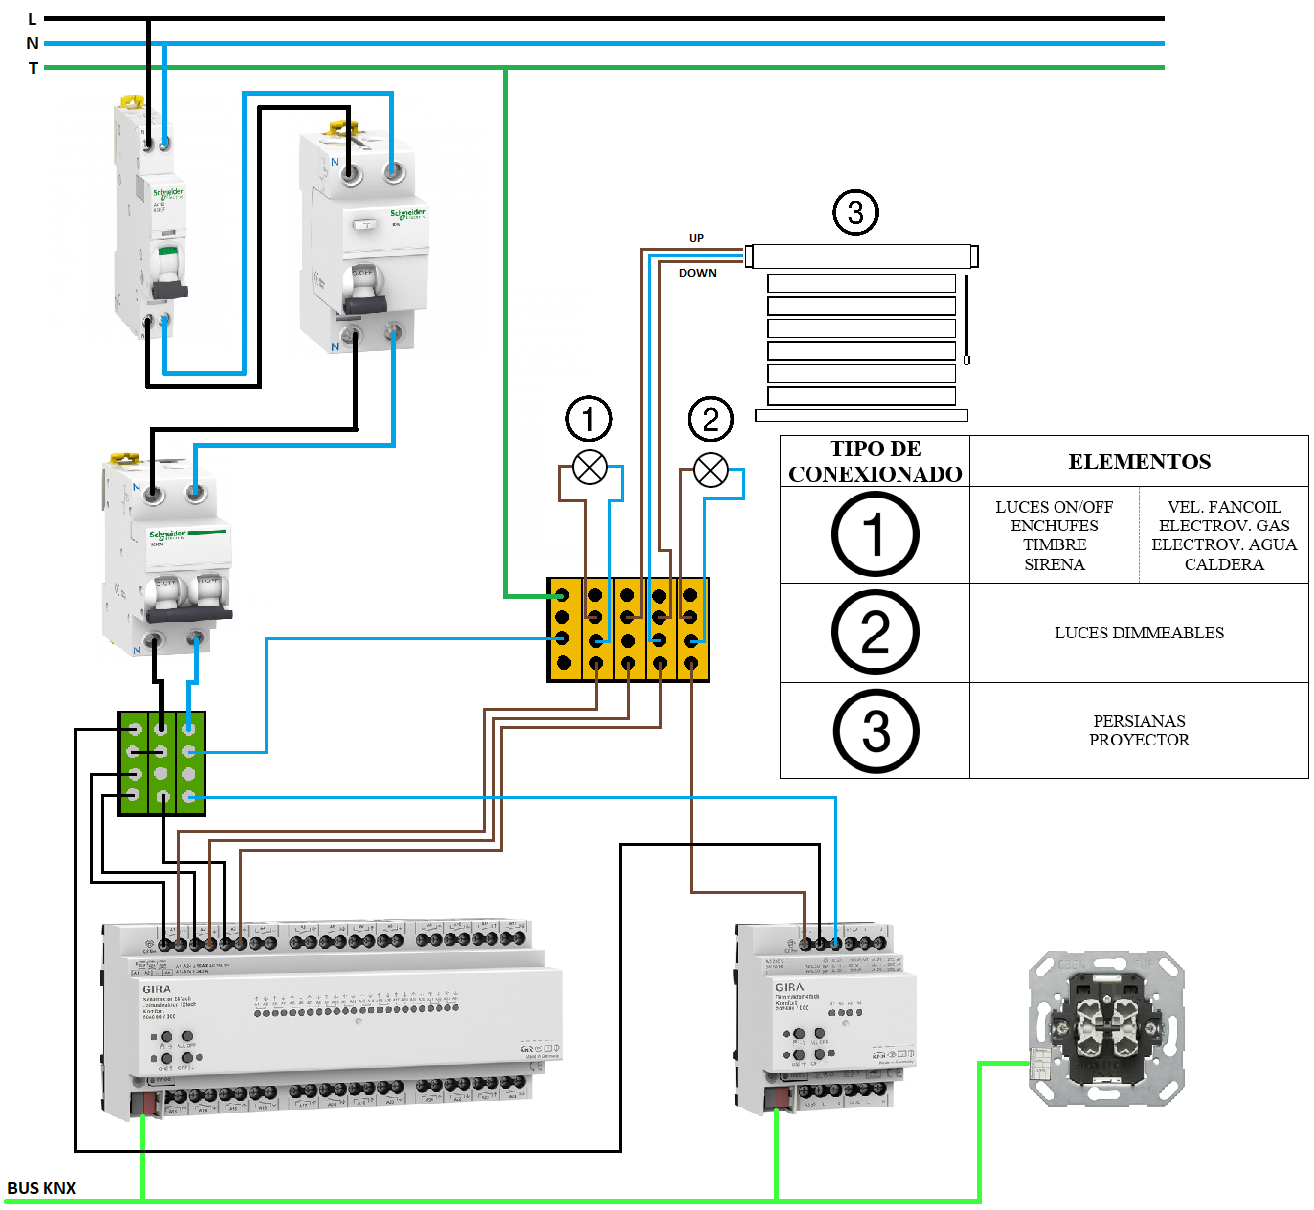
\includegraphics[width=1.15\textwidth]{figures/conex_ilu.png}   
\caption{Conexionado actuadores reguladores y binarios y de persianas}
\label{fig:conex_ilu}
\end{figure}
\end{flushleft}

\begin{itemize}
\item \textbf{Contadores de consumo} \\ \\
Para los módulos de conteo de consumo de agua y gas será necesario contar con las cajas de registro instaladas en la vivienda por la empresa suministradora, ya que este módulo no medirá los caudales de manera directa. Las cajas de registro se encuentran conectadas tanto a la caldera, para el conteo del caudal de gas, como a todas las tomas de agua de la vivienda, e irán emitiendo pulsos SO que serán  cuantificados a través de un optoacoplador y transformados en un número entero a través de un factor de conversión programado en el dispositivo. \\
Por otro lado, los módulos de consumo eléctrico si realizarán el conteo de manera directa a través de los acopladores de corriente instalados en la fase de entrada de cada uno de los circuitos eléctricos que conforman la carga. Estos acopladores realizarán las mediciones mediante el uso del efecto Hall dado en los cables sobre los que se encuentran “abrazados”, por lo que será necesario planificar un espacio en los tubos de cableado que se encuentran en las paredes de la vivienda.
\end{itemize}
\begin{flushleft}
\begin{figure}[H]
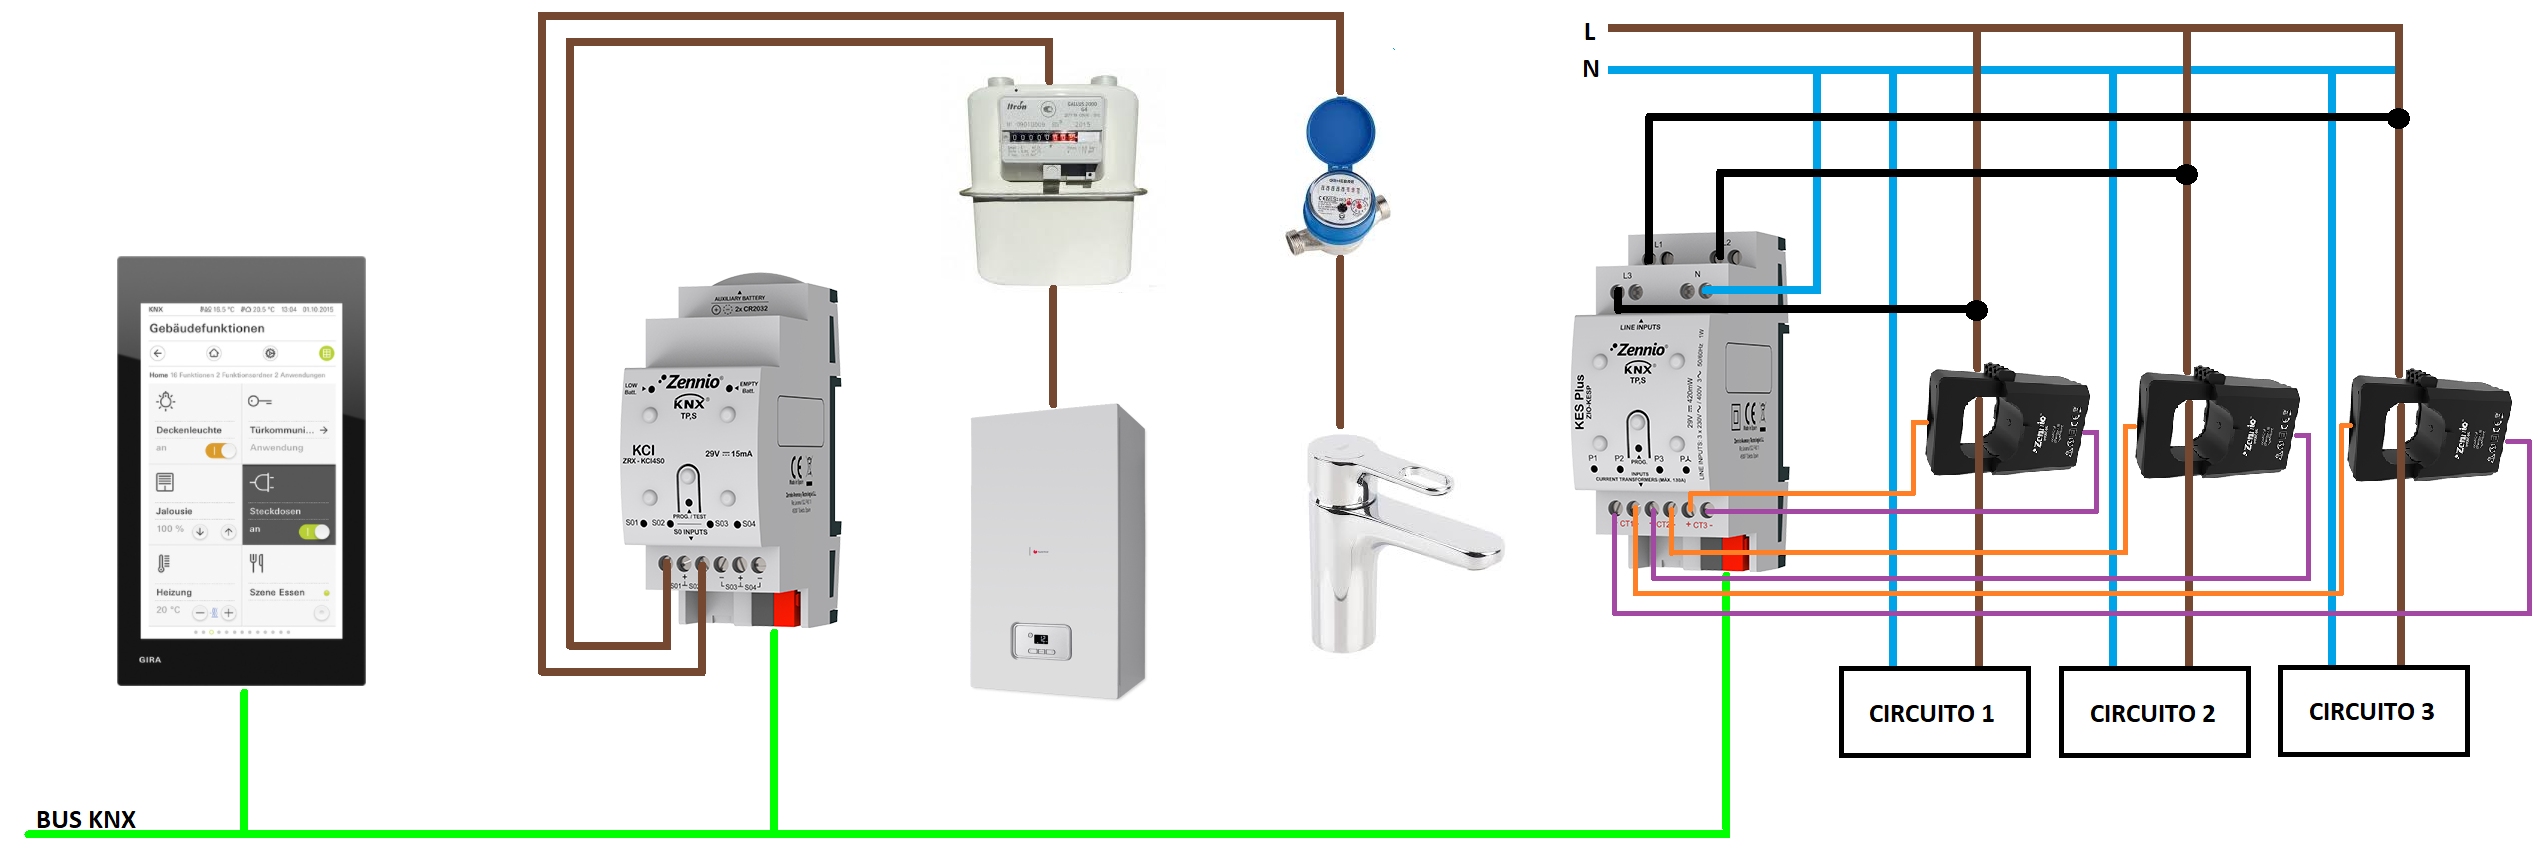
\includegraphics[width=1.15\textwidth]{figures/conex_consumo.png}   
\caption{Conexionado módulos de medidas de consumo}
\label{fig:conex_consumo}
\end{figure}
\end{flushleft}

\begin{itemize}
\item \textbf{} \\ \\
\end{itemize} 